\section{Part 2}
In this section, it was desirable to implement a PID-regulator to keep the level of the tank as desired. The PROFIBUS network contains two slave-nodes contributing us with necessary information to use the master (PLC) to regulate the water level. The valve is used as gain, where the valve opening changes along with the set value (SV). The DP-cell contributed with actual differensial pressure, and after calibration, the actual level of the tank.

In Simatic Manager we used the following blocks; PID (FB41), write to valve (SFC15), read from DP (SFC14) and different data- and function-blocks.

To implement the different blocks we needed the correct addresses. These were found using the programming calculator on the Desktop PC, and as a verification we checked them against old projects.

\begin{figure}[!htb]
    \centering
    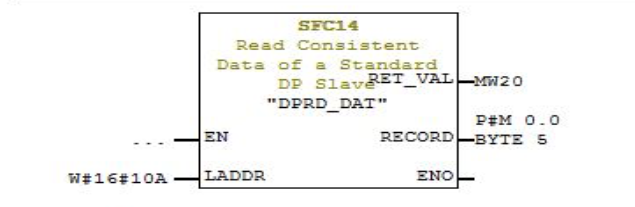
\includegraphics[width=0.9\textwidth]{images/bilde2}
    \caption{SFC14 block}
\end{figure}

\begin{figure}[!htb]
    \centering
    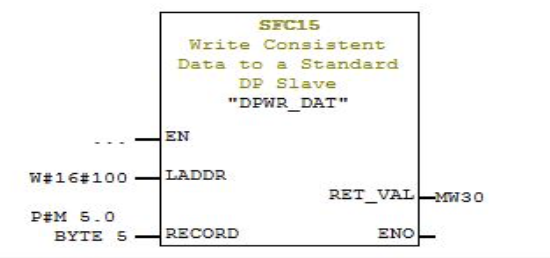
\includegraphics[width=0.8\textwidth]{images/bilde3}
    \caption{SFC15 block}
\end{figure}